
\documentclass{standalone}
\usepackage{tikz}
\usepackage{fp}
\begin{document}
        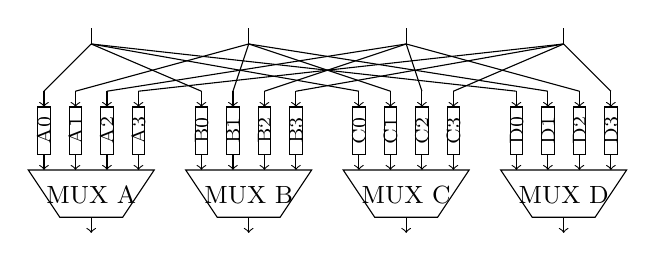
\begin{tikzpicture}[scale=.4]
            \foreach \i/\l in {0/A, 5/B, 10/C, 15/D}{
                \draw[xshift=\i cm] (-2,1) -- (2,1) -- (1,-.5) -- (-1,-.5) -- cycle;
                \node at (\i,.2){\small MUX \l};
                \draw [xshift=\i cm,->](0,-.5) -- (0,-1);
                \foreach \j/\p in {-1.5/0, -.5/1, .5/2,1.5/3}{
                    \draw [xshift = \i cm](\j-.2,1.5) rectangle (\j+.2,3);
                    \node at (\i+\j,2.25)[rotate=90]{\scriptsize \l\p};
                    \draw [xshift = \i cm,->](\j,1.5) -- (\j,1);
                    \draw [xshift = \i cm,->](\j,3.5) -- (\j,3);
                }
            }
            \foreach \i/\j in {0/-1.5, 5/-.5, 10/.5, 15/1.5}{
                \foreach \k in {0, 5, 10, 15}{
                    \draw (\i, 5) -- (\k+\j, 3.5);
                }
                \draw (\i,5) -- (\i, 5.5);
            }
        \end{tikzpicture}
\end{document}
